\documentclass[12pt,a4paper]{article}
\usepackage[utf8]{inputenc}
\usepackage[brazil]{babel}
\usepackage[T1]{fontenc}
\usepackage{amsmath}
\usepackage{amsfonts}
\usepackage{amssymb}
\usepackage{graphicx}
\usepackage{booktabs}
\usepackage{array}
\usepackage{geometry}
\usepackage{hyperref}
\usepackage{float}
\usepackage{xcolor}
\usepackage{multirow}
\usepackage{subcaption}
\usepackage{listings}
\usepackage{helvet}
\renewcommand{\familydefault}{\sfdefault}

\geometry{margin=2.5cm}
\graphicspath{{./figuras/}}

% Remover numeração das seções
\setcounter{secnumdepth}{0}

% Configuração para código R
\lstset{
    language=R,
    basicstyle=\ttfamily\small,
    keywordstyle=\color{blue},
    stringstyle=\color{orange},
    commentstyle=\color{gray},
    numbers=none,
    frame=single,
    breaklines=true,
    backgroundcolor=\color{gray!10},
    showstringspaces=false
}

\hypersetup{
    colorlinks=true,
    linkcolor=blue,
    filecolor=magenta,
    urlcolor=cyan,
}

\begin{document}

% ============================================================================
% INTRODUÇÃO
% ============================================================================
\section{}

\textbf{Aluno:} Gabriel Francelino Voidaleski

\textbf{Curso:} Tecnologia em Análise e Desenvolvimento de Sistemas (TADS)

\textbf{Disciplina:} Biologia Computacional e Sistemas

\vspace{0.5cm}

Este trabalho mostra uma análise dos dados da Organização Mundial da Saúde (OMS) sobre Covid-19 usando grafos. A ideia foi sair da tabela tradicional e usar redes para enxergar melhor conexões entre países, semelhança entre regiões e grupos com comportamento parecido.

% ============================================================================
% 2. BASE DE DADOS
% ============================================================================
\section{Base de Dados Escolhida}

\textbf{Fonte:} World Health Organization (WHO) Covid-19 Dashboard

\textbf{URL:} \url{https://data.who.int/dashboards/covid19/data}

\textbf{Arquivo utilizado:} \texttt{WHO-COVID-19-global-table-data.csv}

\textbf{Descrição:} Base com indicadores globais de Covid-19 por país/região, com casos e óbitos acumulados, além de indicadores recentes.

\begin{lstlisting}
# Carregar dados
who_df <- read.csv("WHO-COVID-19-global-table-data.csv",
                   stringsAsFactors = FALSE,
                   check.names = FALSE,
                   fileEncoding = "UTF-8-BOM")

# Organizar em data.frame e padronizar nomes de colunas
stopifnot(is.data.frame(who_df))
\end{lstlisting}

% ============================================================================
% 2. TÉCNICAS DE VISUALIZAÇÃO
% ============================================================================
\section{Técnicas de Visualização em Rede Escolhidas}

\begin{itemize}
    \item \textbf{Estratégia A:} Rede bipartida Região--País
    \item \textbf{Estratégia B:} Rede de similaridade entre regiões
    \item \textbf{Estratégia C:} Rede de proximidade entre países (k-NN)
    \item \textbf{Estratégia D:} Rede país--país por perfil de carga e letalidade
    \item \textbf{Estratégia E:} Rede bipartida Região--Indicador
\end{itemize}

\begin{lstlisting}
# Exemplo de preparação
who_df$region[is.na(who_df$region) | who_df$region == ""] <- "Unknown"
who_df <- subset(who_df,
                 country != "Global" &
                 !grepl("^International conveyance", country))
\end{lstlisting}

% ============================================================================
% 3. VISUALIZAÇÃO INICIAL
% ============================================================================
\section{Visualização Inicial - Rede Bipartida Região--País}

A primeira visualização foi uma rede bipartida ligando regiões OMS aos países com maior volume de casos acumulados. Essa etapa serviu como uma visão geral inicial dos dados.

\begin{figure}[H]
\centering
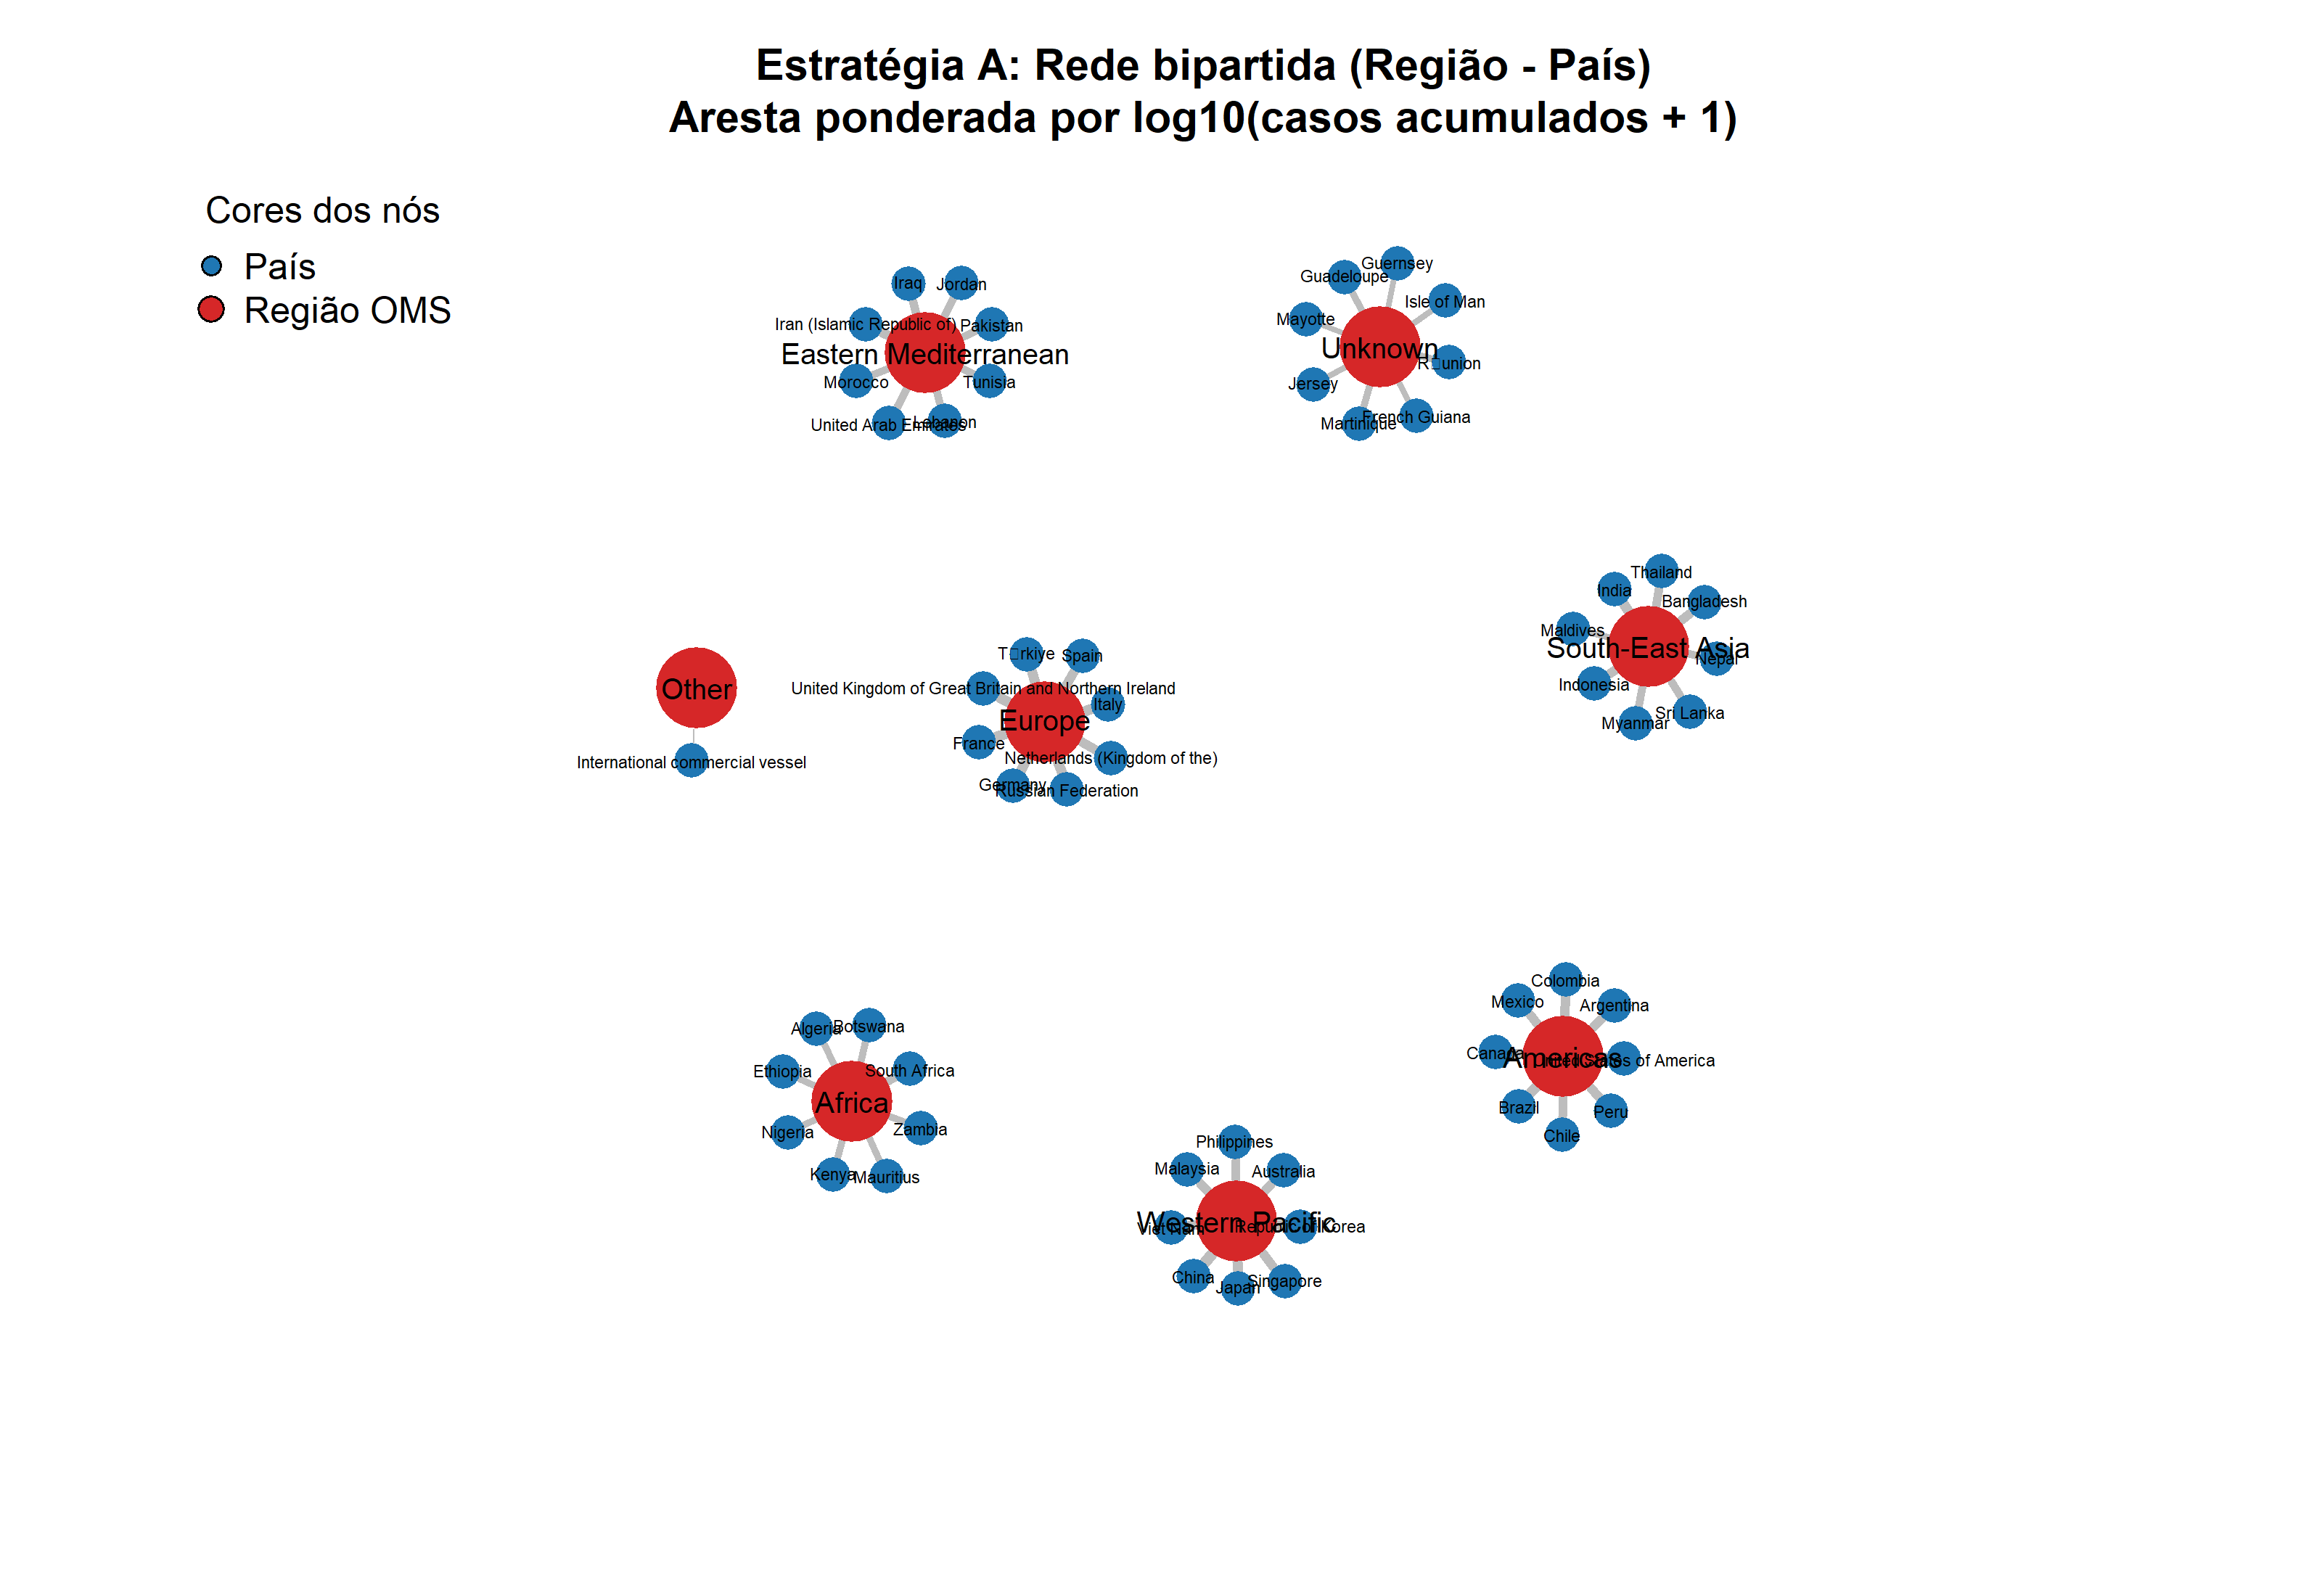
\includegraphics[width=0.98\textwidth]{rede_bipartida_regiao_pais.png}
\caption{Rede bipartida Região--País (Estratégia A)}
\end{figure}

\textbf{Interpretação da Estratégia A (em linguagem simples):}
\begin{itemize}
    \item As regiões aparecem como nós centrais e os países ficam conectados a elas.
    \item Países com mais casos acumulados ficam mais evidentes no desenho.
    \item Fica fácil ver onde a carga de casos está mais concentrada em cada região.
\end{itemize}

% ============================================================================
% 4. MÉTODOS PARA MELHORAR
% ============================================================================
\section{Métodos Aplicados para Melhorar os Resultados}

Depois da visualização inicial, foram aplicadas melhorias para deixar a análise mais clara:

\begin{itemize}
    \item \textbf{Padronização e filtros de completude} para reduzir ruído de valores ausentes.
    \item \textbf{Medições de similaridade} por distância euclidiana em dados escalados.
    \item \textbf{Detecção de comunidades} (Louvain) em redes país--país.
    \item \textbf{Inclusão de CFR} (\textit{case fatality ratio}) na análise de severidade.
    \item \textbf{Legendas e rotulagem} para facilitar leitura visual.
\end{itemize}

\begin{lstlisting}
# Exemplo de medida adicional
who_df$cfr <- ifelse(who_df$cases_total > 0,
                     who_df$deaths_total / who_df$cases_total,
                     NA_real_)
\end{lstlisting}

% ============================================================================
% 5. VISUALIZAÇÕES - RESULTADO OBTIDO
% ============================================================================
\section{Visualizações Produzidas - Resultado Obtido}

\subsection{Estratégia B - Similaridade entre Regiões}
\begin{figure}[H]
\centering
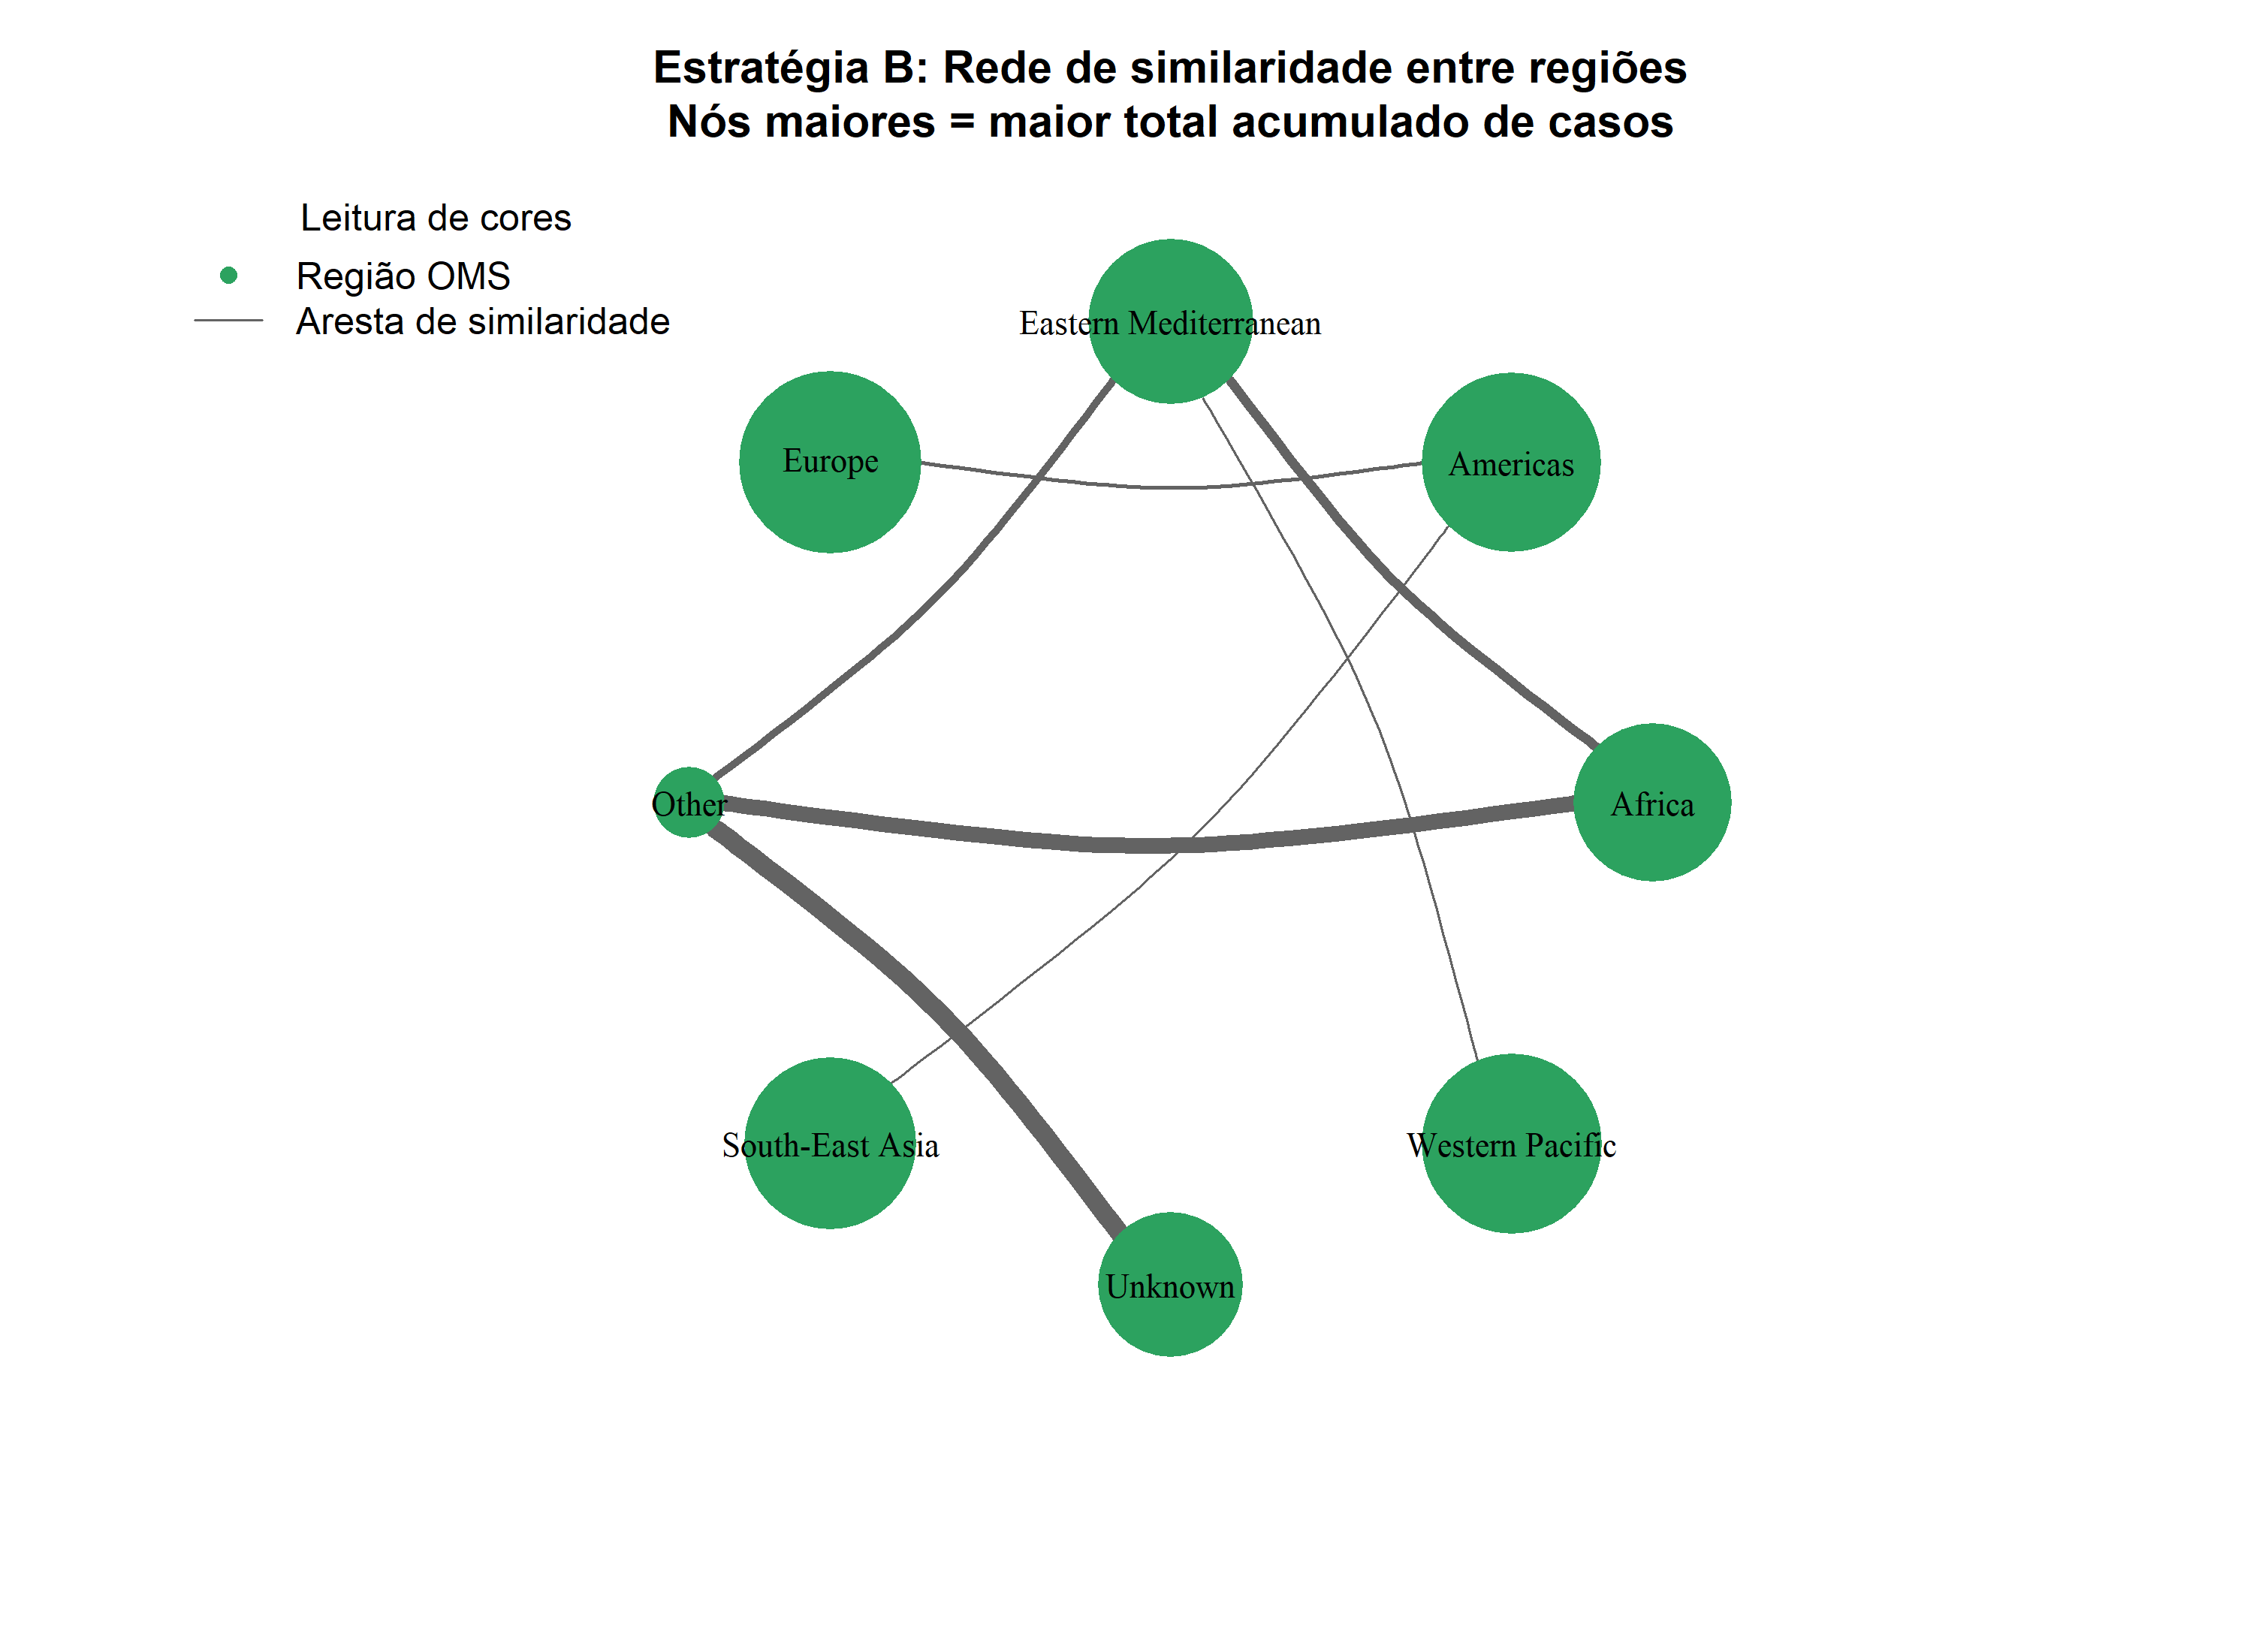
\includegraphics[width=0.90\textwidth]{rede_similaridade_regioes.png}
\caption{Rede de similaridade entre regiões (Estratégia B)}
\end{figure}

\textbf{Interpretação da Estratégia B:}
\begin{itemize}
    \item Cada nó representa uma região da OMS.
    \item Regiões com ligação mais forte têm indicadores médios mais parecidos.
    \item Essa visualização ajuda a comparar regiões rapidamente, sem depender de muitas tabelas.
\end{itemize}

\subsection{Estratégia C - Proximidade entre Países (k-NN)}
\begin{figure}[H]
\centering
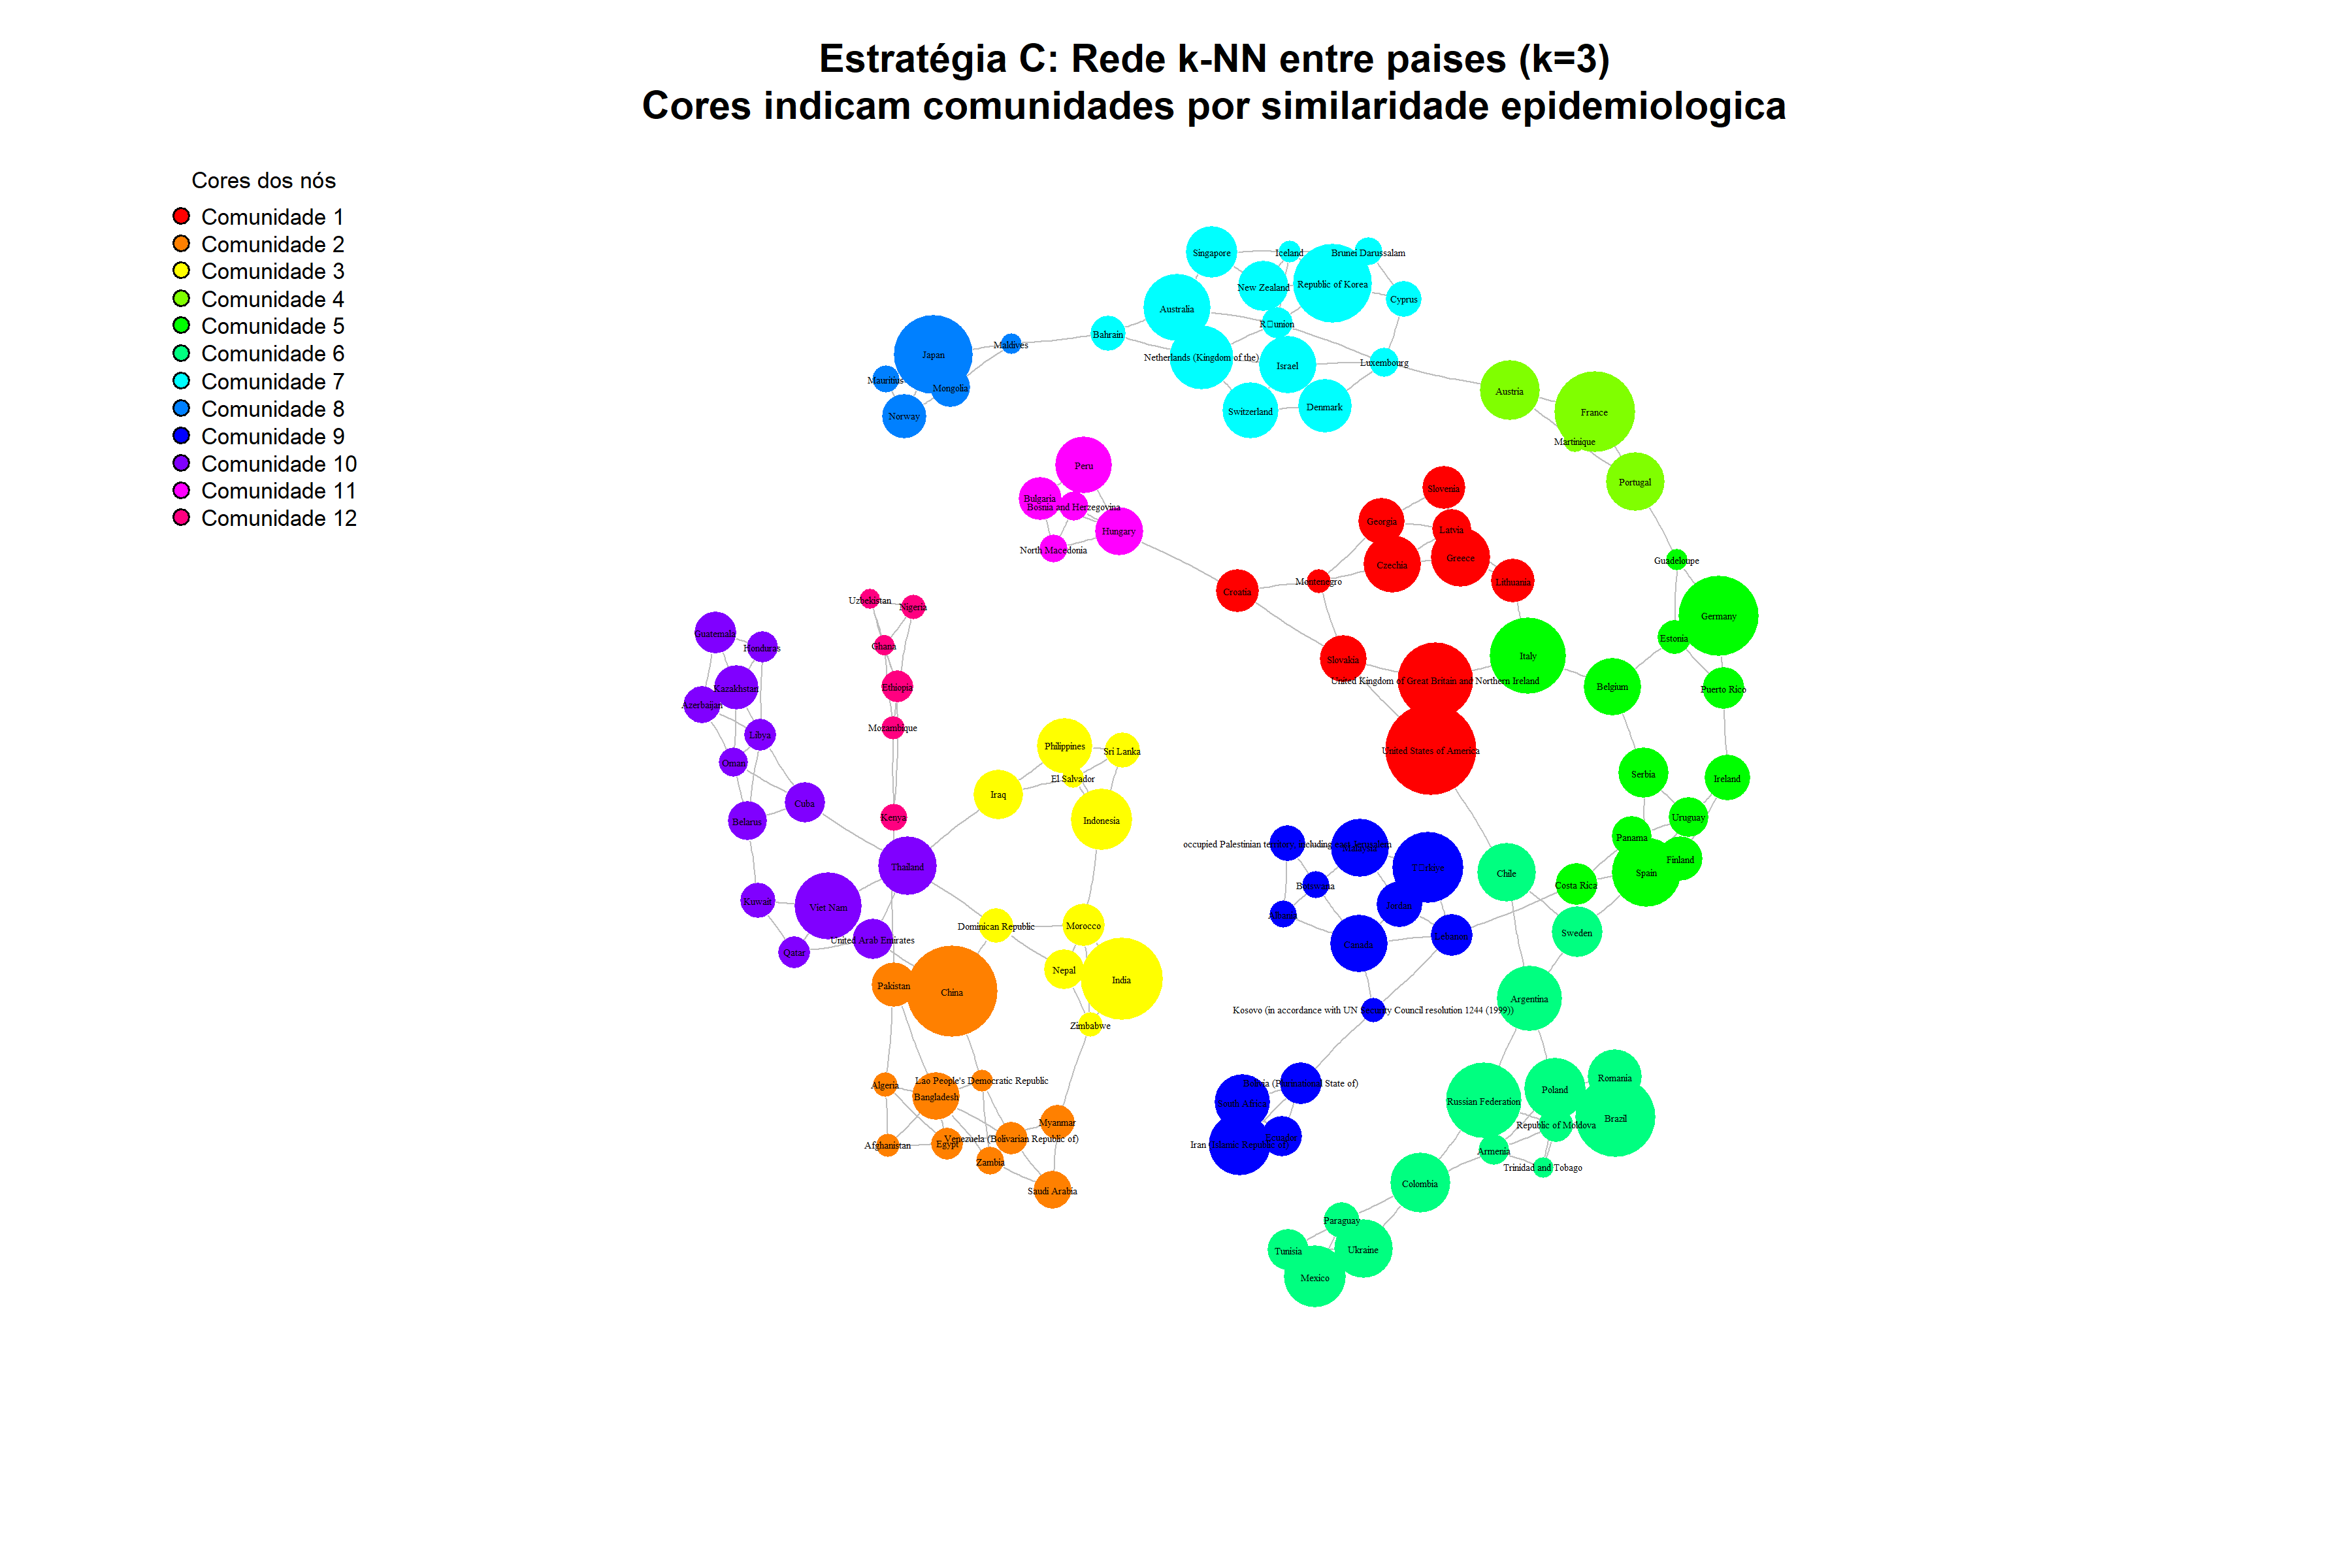
\includegraphics[width=0.98\textwidth]{rede_proximidade_paises_knn.png}
\caption{Rede k-NN entre países com comunidades por cor (Estratégia C)}
\end{figure}

\textbf{Interpretação da Estratégia C:}
\begin{itemize}
    \item Cada país foi conectado aos vizinhos mais parecidos nos indicadores usados.
    \item As cores mostram comunidades (grupos) encontradas automaticamente.
    \item Mesmo países distantes geograficamente podem cair no mesmo grupo se tiverem padrão semelhante.
\end{itemize}

\subsection{Estratégia D - Perfil de Carga e Letalidade}
\begin{figure}[H]
\centering
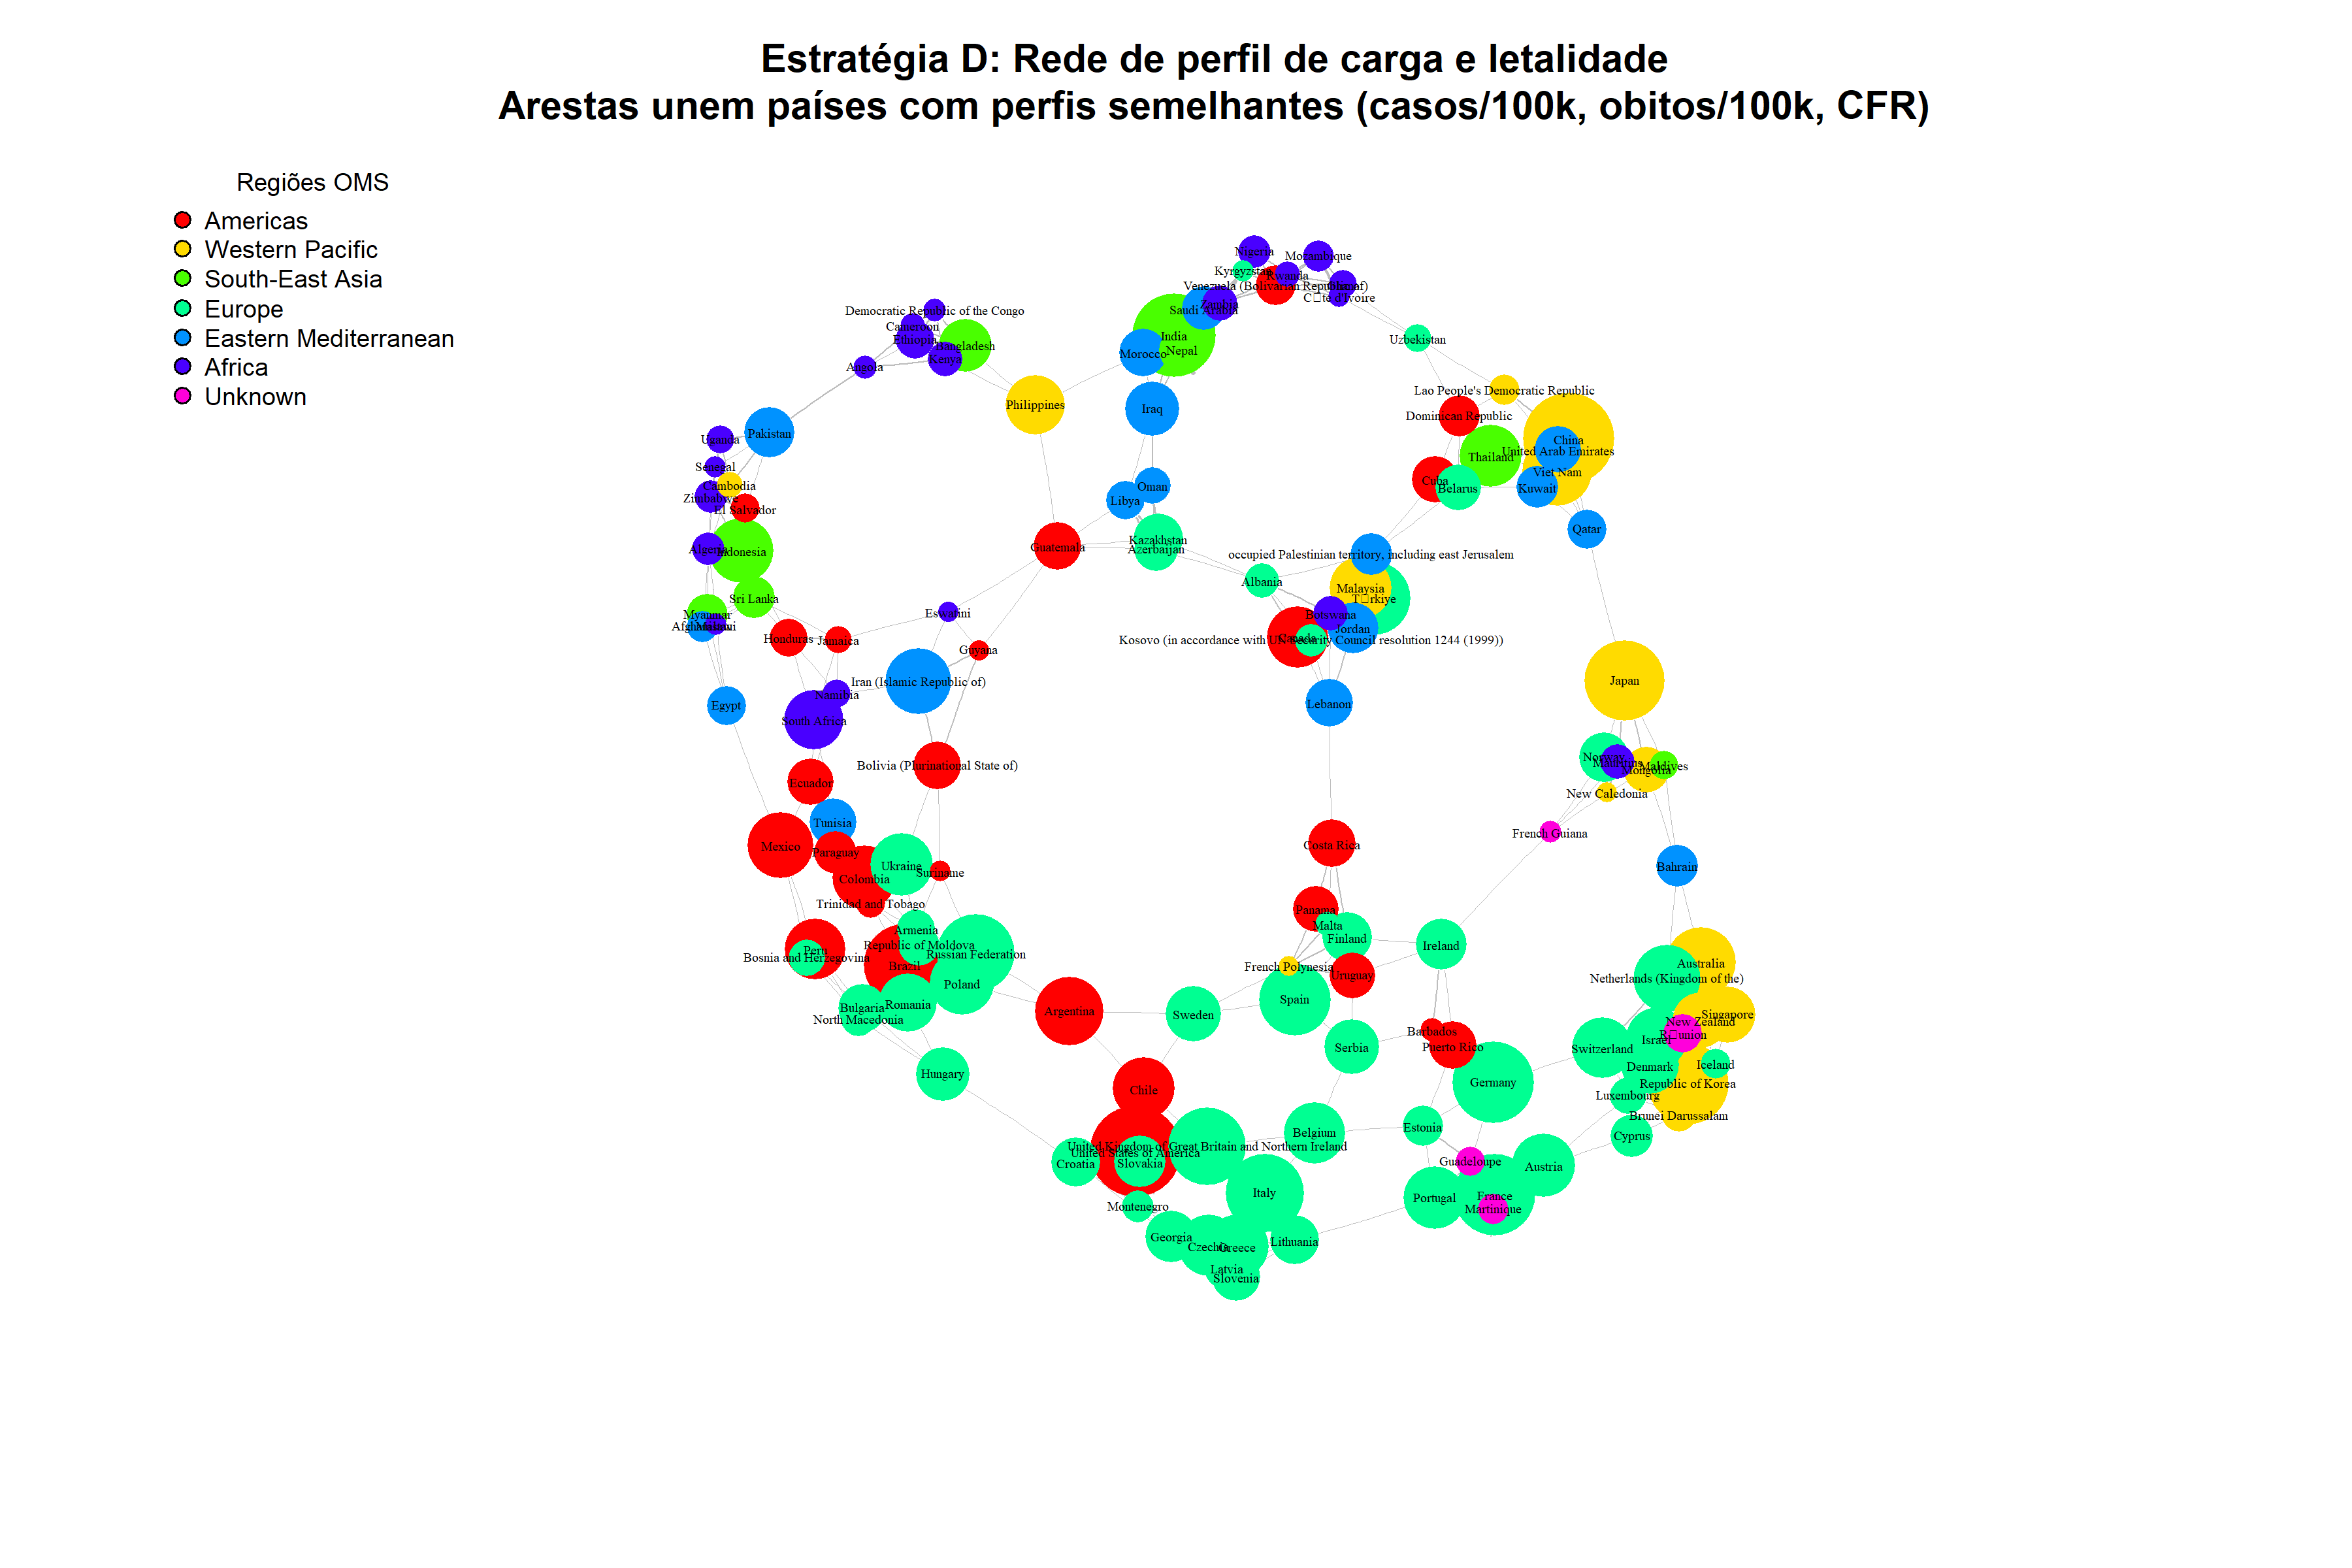
\includegraphics[width=0.98\textwidth]{rede_perfil_letalidade_carga.png}
\caption{Rede país--país com casos/100k, óbitos/100k e CFR (Estratégia D)}
\end{figure}

\textbf{Interpretação da Estratégia D:}
\begin{itemize}
    \item Aqui a comparação junta carga de casos, carga de óbitos e CFR (letalidade).
    \item Isso evita analisar só "quantidade de casos" e traz também uma noção de severidade.
    \item O resultado ajuda a separar países com perfil epidemiológico mais crítico.
\end{itemize}

\subsection{Estratégia E - Assinatura Região--Indicador}
\begin{figure}[H]
\centering
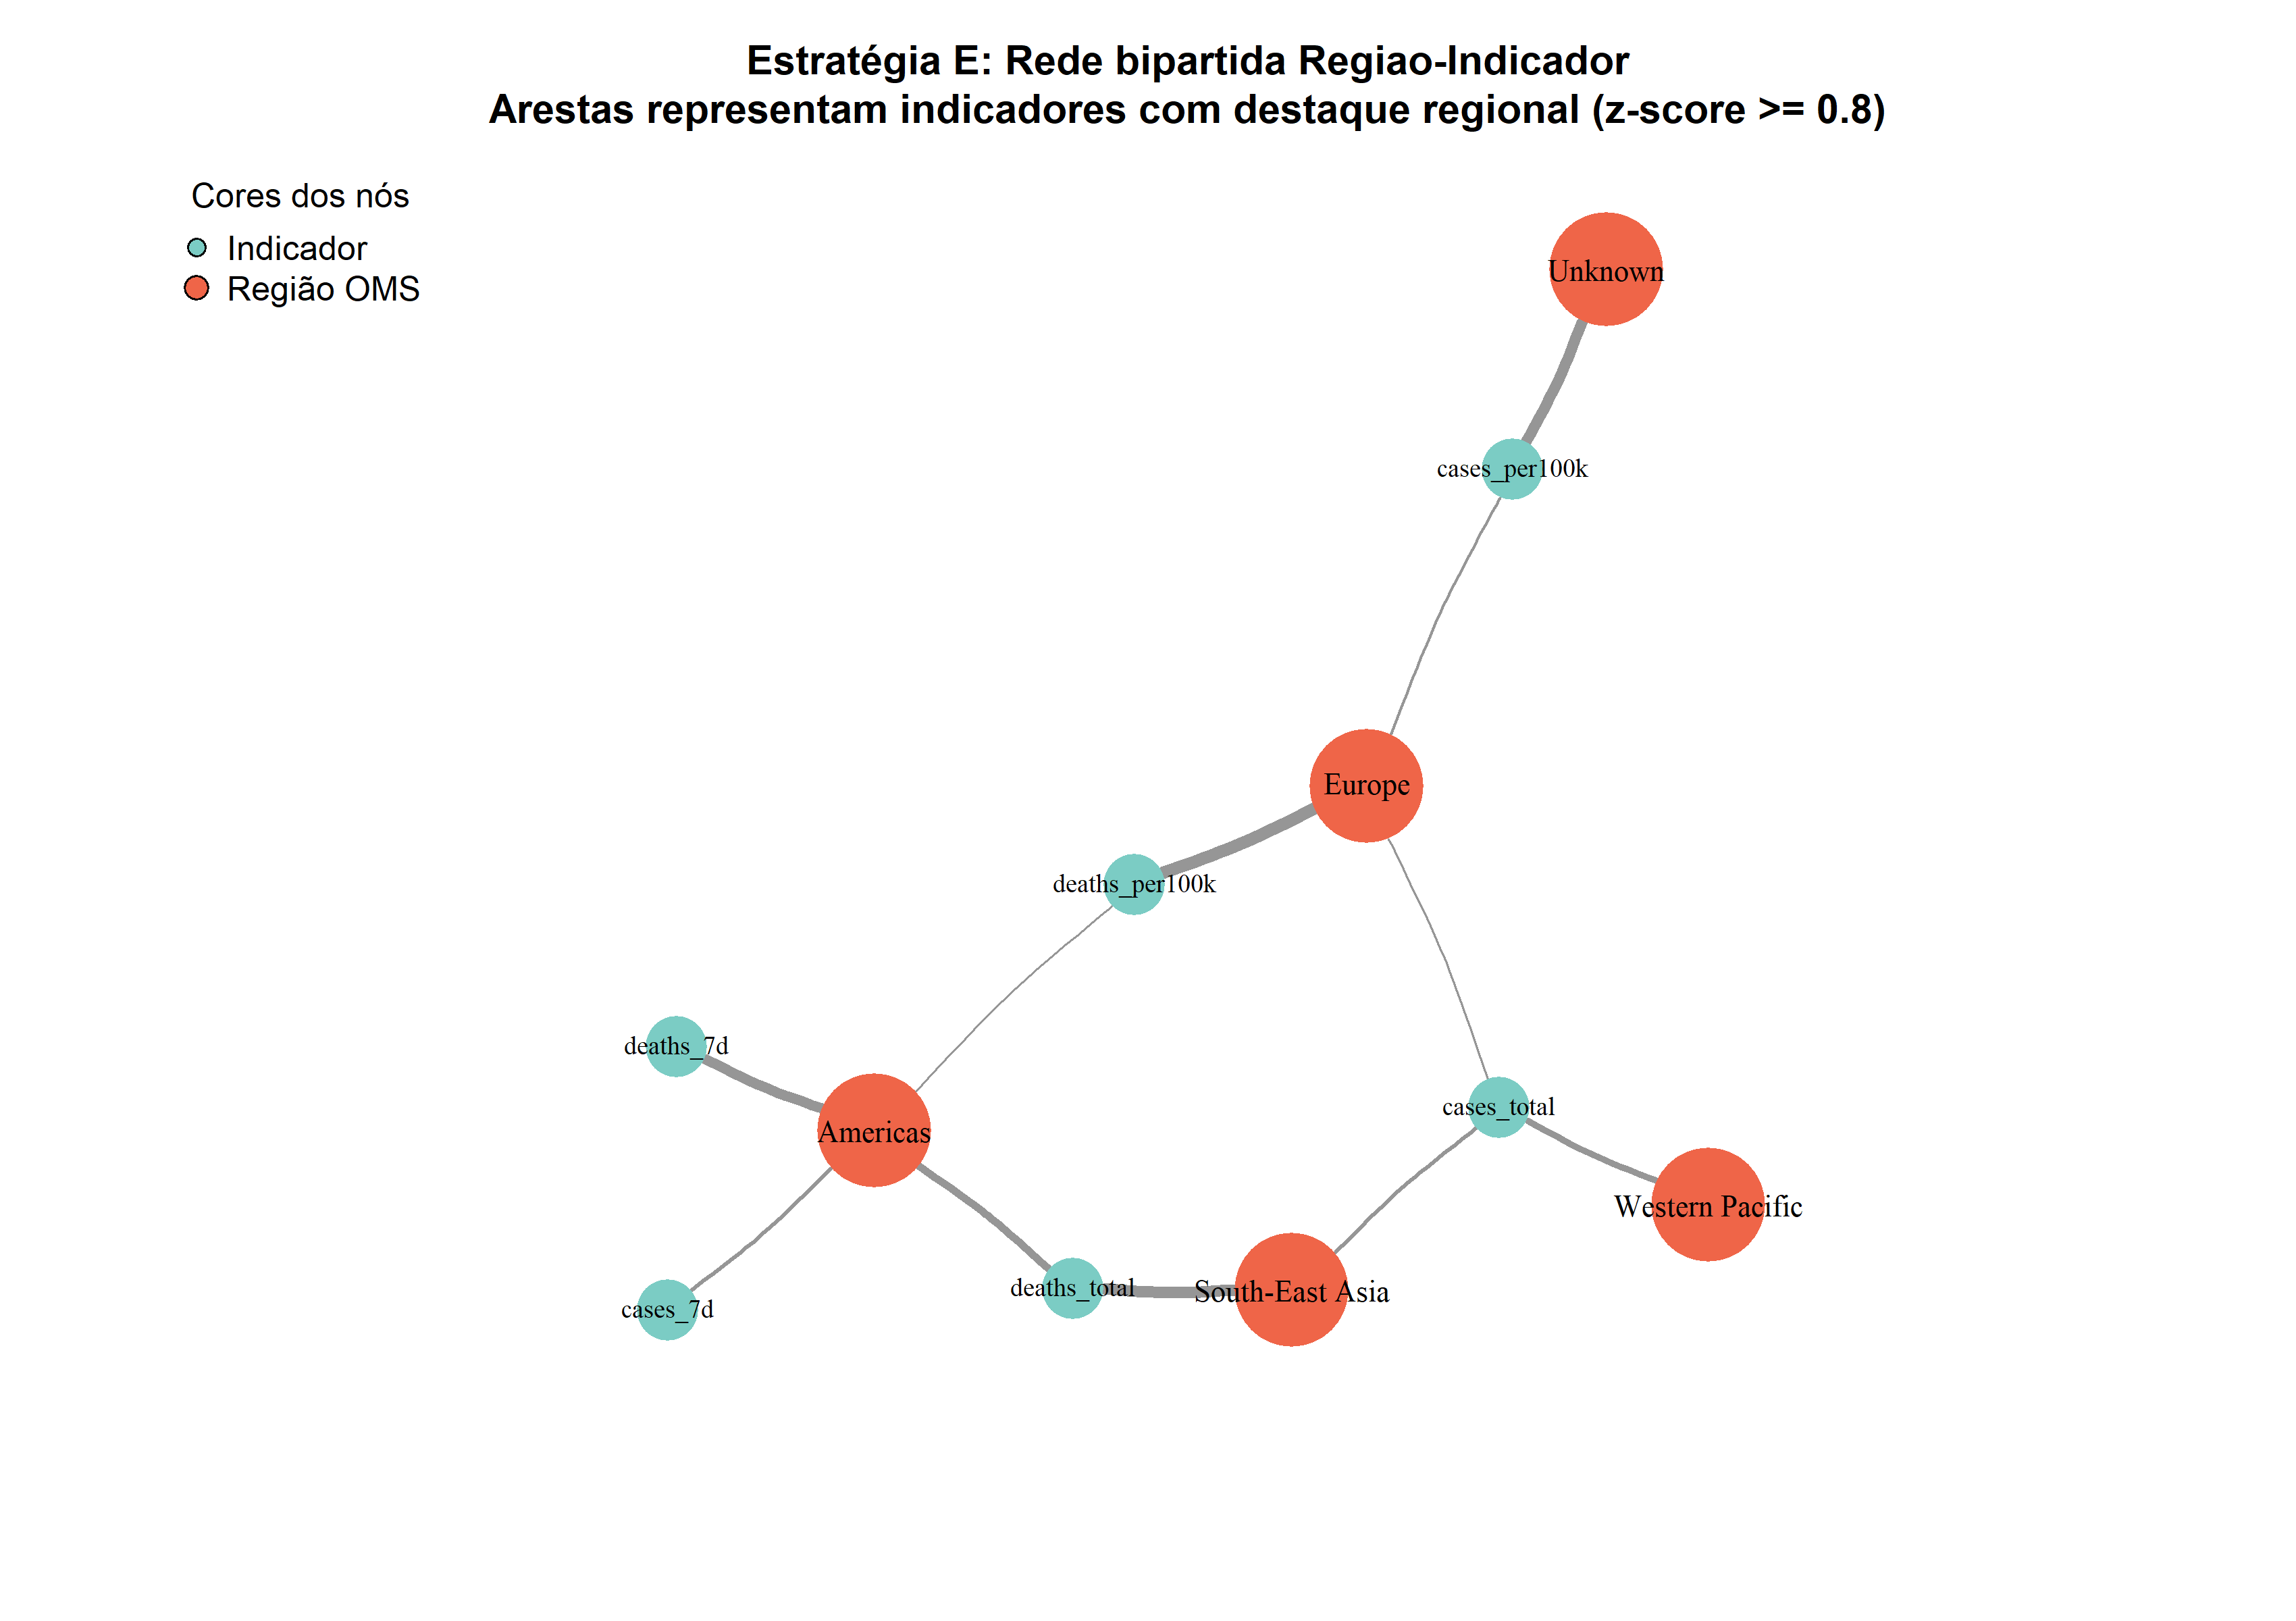
\includegraphics[width=0.98\textwidth]{rede_bipartida_regiao_indicador.png}
\caption{Rede bipartida Região--Indicador por destaque relativo (Estratégia E)}
\end{figure}

\textbf{Interpretação da Estratégia E:}
\begin{itemize}
    \item A rede mostra quais indicadores mais se destacam em cada região.
    \item Funciona como um resumo rápido do "perfil" de cada região.
    \item Facilita comparar prioridades e diferenças regionais de forma visual.
\end{itemize}

\textbf{Padrões observados:}
\begin{itemize}
    \item Regiões com perfis parecidos ficam mais conectadas entre si.
    \item A rede k-NN agrupou países com comportamento semelhante, mesmo quando estão em continentes diferentes.
    \item O uso de CFR deixou mais clara a diferença entre volume de casos e severidade.
    \item A rede Região--Indicador resumiu bem quais métricas mais chamam atenção em cada região.
\end{itemize}

% ============================================================================
% 6. COMPARAÇÃO
% ============================================================================
\section{Comparação dos Resultados}

\begin{table}[H]
\centering
\caption{Resumo Comparativo das Estratégias}
\begin{tabular}{p{2.4cm}p{4.2cm}p{6.3cm}}
\toprule
\textbf{Estratégia} & \textbf{Foco} & \textbf{Principal ganho analítico} \\
\midrule
A & Região--País (bipartida) & Evidencia estrutura de vínculo e concentração de carga \\
B & Região--Região (similaridade) & Compara perfis médios regionais de forma direta \\
C & País--País (k-NN) & Detecta comunidades e agrupamentos de comportamento \\
D & País--País (carga + CFR) & Integra volume e severidade em uma mesma leitura \\
E & Região--Indicador (bipartida) & Resume indicadores de destaque por região \\
\bottomrule
\end{tabular}
\end{table}

\textbf{Conjunto mais informativo:} Estratégias C + D + E (complementares para padrão, severidade e síntese regional)

% ============================================================================
% 7. CONCLUSÃO
% ============================================================================
\section{Conclusão}

No geral, a abordagem com redes deixou a leitura dos dados mais intuitiva e visual. Foi possível identificar relações entre regiões e países, grupos de comportamento semelhante e diferenças de severidade com apoio do CFR.

As cinco visualizações se complementam bem: a Estratégia A dá a visão geral, B e C mostram semelhanças, D destaca severidade e E resume o perfil de cada região.

\end{document}
